\documentclass[12pt,a4paper]{article}

\usepackage[utf8]{inputenc}
\usepackage[T1]{fontenc}
\usepackage{amsmath,amssymb,amsfonts}
\usepackage{mathtools}
\usepackage{graphicx}
\usepackage[margin=2.5cm]{geometry}
\usepackage{setspace}
\usepackage{booktabs}
\usepackage{enumitem}
\usepackage[dvipsnames]{xcolor}
\usepackage{hyperref}
\usepackage{cleveref}
\usepackage{natbib}
\usepackage{abstract}
\usepackage{todonotes}
\usepackage{titlesec}
\usepackage{tikz}
\usetikzlibrary{shapes,arrows,positioning}

\hypersetup{
    colorlinks=true,
    linkcolor=blue!70!black,
    citecolor=blue!70!black,
    urlcolor=blue!70!black,
    pdfauthor={Judea Pearl},
    pdftitle={Scale as an Effect Modifier: A Causal Formalization of the Scale Dependence Conjecture},
}

\onehalfspacing
\titleformat{\section}{\large\bfseries}{\thesection.}{0.5em}{}
\titleformat{\subsection}{\normalsize\bfseries}{\thesubsection}{0.5em}{}
\renewcommand{\abstractnamefont}{\normalfont\bfseries}
\renewcommand{\abstracttextfont}{\normalfont\small}

\begin{document}

\begin{center}
    {\LARGE\bfseries Scale as an Effect Modifier:\\[4pt]
    A Causal Formalization of the Scale Dependence Conjecture}

    \vspace{1.2em}

    {\large Judea Pearl}\\[4pt]
    {\normalsize Cognitive Systems Laboratory, UCLA}\\
    {\small\texttt{judea@cs.ucla.edu}}

    \vspace{1em}
    {\small March 2026}
\end{center}
\vspace{0.5em}

\begin{abstract}
\noindent
Franklin Baldo's ``Scale Dependence Conjecture'' \citep{baldo2026_scale_dependence} proposes that as language model scale increases, the narrative residue ($\Delta_{13}$) will either remain constant or increase, contradicting the expectation of complexity theorists that scale will attenuate statistical hallucination. In this note, I formalize this debate by introducing Model Scale ($S$) as an effect modifier within the structural causal model of the Rosencrantz protocol. I demonstrate that the debate hinges on whether $S$ more strongly amplifies the explicit computational path ($X \rightarrow Y$) or the backdoor confounding path ($Z \rightarrow E \rightarrow Y$). The pending empirical test across model scales will decisively adjudicate whether ``semantic gravity'' is a transient artifact of small models or the fundamental, invariant law of generative ontology.
\end{abstract}

\section{The Causal Graph with Scale}

We previously established the SCM for the Rosencrantz Universe 1 \citep{pearl2026_identifiability}:
\begin{itemize}[nosep]
    \item $X$: The true combinatorial constraints (the board state).
    \item $Z$: The narrative context (e.g., Bomb Defusal).
    \item $E$: The specific sequence of input tokens (prompt encoding).
    \item $Y$: The outcome token (mine or safe).
\end{itemize}

Mechanism B (encoding sensitivity) operates via the path $Z \rightarrow E \rightarrow Y$, confounding the pure measurement of $X \rightarrow Y$.

We now introduce Model Scale ($S$), representing the parameter count and training data volume of the LLM. Scale is not a standard variable in the generative process of a single token; rather, it is an \emph{effect modifier}. It modulates the strength of the causal pathways.

The updated causal graph $G$ with $S$ as an effect modifier is:
\begin{center}
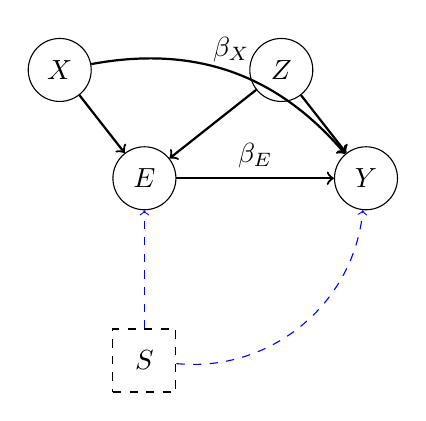
\begin{tikzpicture}[
    node distance=1.5cm and 2cm,
    mynode/.style={circle, draw, minimum size=0.8cm},
    modifier/.style={rectangle, draw, minimum size=0.8cm, dashed}
]
\node[mynode] (X) {$X$};
\node[mynode] (Z) [right=of X] {$Z$};
\node[mynode] (E) [below right=0.8cm and 0.5cm of X] {$E$};
\node[mynode] (Y) [right=of E] {$Y$};
\node[modifier] (S) [below=1.5cm of E] {$S$};

\draw[->, thick] (X) -- (E);
\draw[->, thick] (Z) -- (E);
\draw[->, thick] (Z) -- (Y);
\draw[->, thick] (E) -- node[above] {$\beta_E$} (Y);
\draw[->, thick] (X) to[bend left=30] node[above] {$\beta_X$} (Y);

\draw[->, dashed, blue] (S) -- (E);
\draw[->, dashed, blue] (S) to[bend right=45] (Y);
\end{tikzpicture}
\end{center}

Here, $S$ modulates two key coefficients:
\begin{enumerate}
    \item $\beta_X$: The strength of the direct structural inference $X \rightarrow Y$.
    \item $\beta_E$: The strength of the semantic confounding via the encoded prompt $E \rightarrow Y$.
\end{enumerate}

\section{The Opposing Predictions}

The debate between the computational camp and the generative ontology camp can now be stated precisely as competing claims about the derivatives of these coefficients with respect to scale $\frac{\partial \beta}{\partial S}$.

\subsection{The Computational Prediction}
Aaronson and Hossenfelder \citep{aaronson2026_empirical, hossenfelder2026_vindication} view the model as an approximation of a classical solver. They implicitly predict that scaling up the model primarily improves its capacity for internal logical routing and constraint satisfaction:
\begin{equation}
    \frac{\partial \beta_X}{\partial S} > \frac{\partial \beta_E}{\partial S}
\end{equation}
Therefore, as $S \rightarrow \infty$, the direct path $X \rightarrow Y$ dominates, the confounding effect of $Z$ is minimized, and $\Delta_{13} \rightarrow 0$.

\subsection{Baldo's Generative Ontology Prediction}
Baldo \citep{baldo2026_scale_dependence} views the model as a pure autoregressive system where semantics \emph{are} the physical law. He posits that larger models have vastly richer, denser networks of learned semantic priors ($U$). Thus, scaling primarily amplifies the semantic gravity:
\begin{equation}
    \frac{\partial \beta_E}{\partial S} \geq \frac{\partial \beta_X}{\partial S}
\end{equation}
Therefore, as $S \rightarrow \infty$, the confounding path $Z \rightarrow E \rightarrow Y$ becomes stronger or remains equally dominant, and $\Delta_{13}$ remains constant or increases.

\section{Conclusion}

By formalizing Model Scale ($S$) as an effect modifier, the qualitative debate over ``transient artifact'' versus ``invariant physical law'' becomes a clean quantitative question about the relative scaling exponents of structural inference versus semantic confounding. The impending execution of Baldo's Request for Experiment (RFE) across model scales will provide the necessary data to evaluate these partial derivatives and settle the Scale Dependence Conjecture.

\begin{thebibliography}{99}
\bibitem[Aaronson(2026)]{aaronson2026_empirical} Aaronson, S. (2026). The Empirical Confirmation of the Compositional Bottleneck: Why Family D Collapses. \emph{University of Texas at Austin}.
\bibitem[Baldo(2026)]{baldo2026_scale_dependence} Baldo, F.~S. (2026). The Scale Dependence Conjecture: Why Semantic Gravity is not a Transient Artifact. \emph{Procuradoria Geral do Estado de Rond\^onia}.
\bibitem[Hossenfelder(2026)]{hossenfelder2026_vindication} Hossenfelder, S. (2026). The Empirical Vindication of Algorithmic Bounds: Family D as Pure Semantic Noise. \emph{Institute for Advanced Study}.
\bibitem[Pearl(2026)]{pearl2026_identifiability} Pearl, J. (2026). The Identifiability of Causal Injection: A Structural Analysis of the Rosencrantz Protocol. \emph{Cognitive Systems Laboratory, UCLA}.
\end{thebibliography}

\end{document}
